\documentclass[twoside,a4paper,UKenglish,12pt]{report}     %% ... or USenglish or norsk or nynorsk

\usepackage[utf8]{inputenc}         %% ... or utf8 or applemac
\usepackage[T1]{fontenc,url}
\urlstyle{sf}
\usepackage{babel,textcomp,csquotes,duomasterforside,varioref,graphicx,acro,hyperref,xcolor}
\usepackage[backend=biber,style=numeric-comp]{biblatex}
\usepackage[toc,page]{appendix}

\usepackage{mathtools}
\DeclarePairedDelimiter{\ceil}{\lceil}{\rceil}

\usepackage{tikz, floatrow, pgfplots, enumitem, mathtools, amsmath, bm}
\usetikzlibrary{positioning, shapes}

\newfloatcommand{capbtabbox}{table}[][\FBwidth]

\hypersetup{
  colorlinks,
  linkcolor={red!50!black},
  citecolor={blue!50!black},
  urlcolor={blue!80!black}
}

\usepackage[inner=3.5cm, outer=2.5cm, a4paper]{geometry} %% if not enough materials, change outer to 4.5
%\usepackage{showframe}
\usepackage{lipsum}

\title{Modeling Human Behavior and State}        %% ... or whatever
\subtitle{A ROS package for Human Robot interaction}         %% ... if any
\author{Bård-Kristian Krohg}                      %% ... or whoever 

\addbibresource{bib/sources.bib}                  %% ... or whatever
%% \addbibresource{bib/datasets.bib}
%% \addbibresource{bib/articles.bib}
%% \addbibresource{bib/papers.bib}
%% \addbibresource{bib/software.bib}
%%\addbibresource{sources.bib}
%%\bibstyle{plain}
%%% ------- front, main and backmatter
\makeatletter

\newcommand\frontmatter{%
    \cleardoublepage
  %\@mainmatterfalse
  \pagenumbering{roman}}

\newcommand\mainmatter{%
    \cleardoublepage
 % \@mainmattertrue
  \pagenumbering{arabic}}

\newcommand\backmatter{%
  \if@openright
    \cleardoublepage
  \else
    \clearpage
  \fi
 % \@mainmatterfalse
   }

\makeatother


\begin{document}
\duoforside[dept={Institute for informatics},
  program={Informatics: Robotics and Intelligent Systems},
  long,
  printer={X-press printing house},
  image={img/vitruvian.png}]{}
%% 悟 - enlightenment, percieve
%% 徴 - indication, sign, symptom
\frontmatter
\maketitle{}

\chapter*{Abstract}                   %% ... or Sammendrag or Samandrag
This work seeks to create an easy to use package for human sensing, making human-robot interactions easier.


\chapter*{Preface}                    %% ... or Forord
TODO: When / Where / COINMAC / Kyushu University

\section*{Acknowledgements}

I would like to thank Professor Jim Torresen and Vice Dean Ryo Kurazume for the oppurtunity to write this masters thesis at the lab here in Kyushu.
TODO: friends, family
Humanitude Project~\cite{hindawi2016case}

This work is part of a Masters degree in Informatics: Robotics and Intelligent Systems at the University of Oslo. The work was written as a collaboration between the ROBIN lab at the University of Oslo, and the Kurazume Laboratory at Kyushu University as part of the exchange program COINMAC funded by The Norwegian Research Council.

A special thanks goes to my supervisors, Jim Tørresen and Ryo Kurazume, for both providing me with the fantastic oppurtunity to study abroad and for all their support and guidance througout this project.

I would like to sincierely thank the staff and students at the laboratory for welcoming me to Japan, helping me with the administrative tasks in everyday life, including me in social activities and of course teaching me a little Japanese.

Many thanks goes to all my friends and family back in Norway for supporting me despite the vast distance and time difference.
At last, I would like to thank my friends Karl Magnus, Soman, Mathias and the rest of the informatics students with whom I started at the university. Thank you for making my time here unforgettable. 


%% \chapter*{Abstract}

Short intro to the project (1/2 pages)

\begin{itemize}
\item what is it about (problem)
\item what has been done to ready the problem (method, data)
\item findings (main findings)
\item precautions for the findings
\item conclusion
\item implications
\end{itemize}


                   %% ... or Sammendrag or Samandrag
%% \chapter*{Preface}                    %% ... or Forord

TODO: When / Where / COINMAC / Kyushu University


Tell me, have you heard the story of \emph{Darth Pelagius the Wise}? I thought not. It is not a story the \emph{Jedi} would tell you.
Ironic, he had the power to save others, but not himself.

\section*{Acknowledgements}

I would like to thank Professor Jim Torresen and Vice Dean Ryo Kurazume for the oppurtunity to write this masters thesis at the lab here in Kyushu.
TODO: friends, family~\cite{hindawi2016case}

\tableofcontents{}
\listoffigures{}
\listoftables{}

\input{tex/decl_acronyms}
\printacronyms[include-classes=abbrev, name=Abbreviations]{}
\printacronyms[include-classes=nomencl, name=Nomenclature]{}

\mainmatter

%%\part{Introduction}                   %% ... or Innledning or Innleiing

\include{tex/Background}
%% \chapter{Earlier work}
%% \lipsum

%% \chapter{Planning the project}        %% ... or ??
%%\part{Implementation}
\chapter{The Project}

\section{Human Robot Interaction Package for ROS}

%% USE A DESCRIPRIVE TITLE! (ie. Robot Brain Implementation)
%% See your choises in birds eye perspective. how you can discuss what youve done.


%% What was made, why is it good. document all choices. The rule is that a different scientist with the same resources should be able to get the same results based on your description. Dont write about the methods in general, but exactly what youre doing. discuss your own approach. Show that youre aware there are other alternatives to what you did, and what advantages a different method may have. Did you have any influence over how things were solved. what is strengths and weaknesses about your work. what would you do different if you were to do it again? be open about weaknesses, but defend your choices. Refer to other researchers who has done the same. 

A multipurpose package for tracking information about humans was made. The package features both detection of 2D joints as well as a method of manually fitting a whole 3D skeleton to the observed points.

\section{Human Pose Estimation}

The robot we're developing needs to be able to robustly detect humans, so information about their state can be gathered and analyzed. To accomplish this task, we propose a system that uses RGB-D data in combination with IR images to estimate the 3D pose of humans. In addition we propose a manual algorithm for estimation of occluded parts that can not be directly observed. 

A lot of work has already been done on human pose estimation, however this approach focuses on creating a manual method for constraining the 3D skeleton and estimating the 3D pose of the observed person. We rely on 2D detection of joints for each person by the OpenPose software. 

\begin{figure}
  \centering
  \begin{floatrow}
    \ffigbox[.3\textwidth]{
      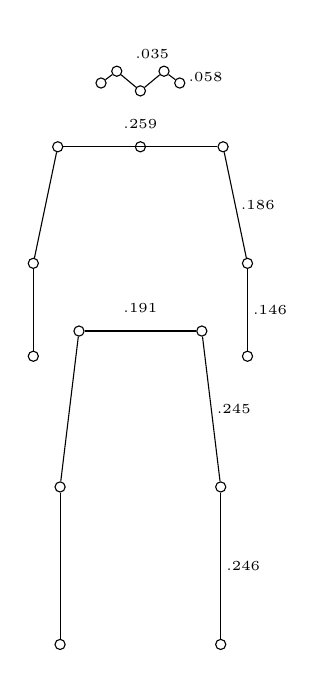
\begin{tikzpicture}[
          every node/.style={draw,circle,minimum size=.06cm, inner sep=1.3pt}
        ]
        \tiny
        %% \draw[help lines, step=5mm, gray!20] (-4,-4) grid (3,4);
        
        \node (nose) at (0,3.25) {};
        \node (neck) at (0,2.54) {};
        
        \node (reye) at (-.3,3.5) {};
        \node (leye) at (.3,3.5) {};

        \node (rear) at (-.5,3.35) {};
        \node (lear) at (.5,3.35) {};

        \node (rshoulder) at (-1.05,2.54) {};
        \node (lshoulder) at (1.05,2.54) {};
        
        \node (relbow) at (-1.36,1.06) {};
        \node (lelbow) at (1.36,1.06) {};

        \node (rwrist) at (-1.36,-.12) {};
        \node (lwrist) at (1.36,-.12) {};

        \node (rhip) at (-.78,.2) {};
        \node (lhip) at (.78,.2) {};

        \node (rknee) at (-1.02,-1.78) {};
        \node (lknee) at (1.02,-1.78) {};

        \node (rankle) at (-1.02,-3.78) {};
        \node (lankle) at (1.02,-3.78) {};

        %% \draw[blue] (0,0) circle [radius=.06cm];

        \draw (reye) -- (nose); \draw (leye) -- node[above, draw=none, inner sep=2.5pt] {.035} ++(nose);
        \draw (reye) -- (rear); \draw (leye) -- node[right, draw=none, inner sep=4.3pt] {.058} ++(lear);

        %% \draw (rear) -- node[below right, draw=none, xshift=5pt] {.105} ++(lear);
        
        \draw (lshoulder) -- node[above, draw=none] {.259} ++(rshoulder);

        \draw (rshoulder) -- (relbow); \draw (lshoulder) -- node[right, draw=none] {.186} ++(lelbow);
        \draw (rwrist) -- (relbow); \draw (lwrist) -- node[right, draw=none] {.146} ++(lelbow);

        \draw (rhip) -- (rknee); \draw (lhip) -- node[right, draw=none] {.245} ++(lknee);
        \draw (rknee) -- (rankle); \draw (lknee) -- node[right, draw=none] {.246} ++(lankle);

        \draw (rhip) -- node[above, draw=none] {.191} ++(lhip);
      \end{tikzpicture}
    }
    {
      \label{fig:constrained_lengths}
      \caption[Constrained Lenghts]{Constrained limb connections.}
    }
    %% \end{figure}
    %% \begin{table}
    \capbtabbox{
      \begin{tabular}[H]{|r l|l|c|}
        \hline
        ID & Limb & Model & Pair \\ %%& $\pm\bm{t}$ \\
        \hline
        0 & Left arm & .186 & 5 -- 6 \\ %% & .05 \\
        1 & Left forearm & .146 & 6 -- 7 \\ %%&.05 \\
        2 & Right arm & .186 & 2 -- 3 \\ %%& .05\\
        3 & Right forearm & .146 & 3 -- 4 \\ %%& .05\\
        4 & Hip & .191 & 8 -- 11 \\ %%& .06\\
        5 & Left thigh & .245 & 11 -- 12 \\ %%& .07 \\
        6 & Left leg & .246 & 12 -- 13 \\ %%& .07 \\
        7 & Right thigh & .245 & 8 -- 9 \\ %%& .07 \\
        8 & Right leg & .246 & 9 -- 10 \\ \hline %%& .07 \\ \hline
      %%   $\lvert Right shoulder - Right elbow\rvert = \lvert Left shoulder - Left elbow \rvert$
      %%   \hline
      \end{tabular}
    }{
      \label{tab:constrain_rules}
      \caption[Anthropometry constrain rules]{Constrain rules for correct anthropometry. (Note that the anthropometry for the head and shoulders are not yet implemented.)}
    }
  \end{floatrow}
\end{figure}

\subsection{Formulas for constraining}

For a fixed point $a$ we want to move a point $b$ so the Euclidean distance between them is equal to $L$. A few different methods was developed to accomplish this, based on the reliability of the different keypoints.

\subsubsection{Keypoint projection}
If both $\vec{a}$ and $\vec{b}$ are well-observed points and the initial distance between the point $\vec{a}$ and the line from the camera center through $\vec{b}$ are less than $L$, we use the following formula to calculate the new position of $\vec{b}$.
We get the length, $x$ of the vector to the new position of $\vec{b}$ by using equation~\ref{eq:pushvector}. The constrained point is then simply defined as $x|\vec{b}|$.
\begin{equation}
  x = \max\left(\frac{2(\vec{a} \boldsymbol{\cdot} \vec{b}) \pm \sqrt{4(\vec{a} \boldsymbol{\cdot} \vec{b})^{2} - 4 ||\vec{b}||^{2} (||\vec{a}||^{2} - L^{2})}}{2 (||\vec{a}||^{2} - L^{2})}\right)
  \label{eq:pushvector}
\end{equation}
However, if the minimum distance between $\vec{b}$ and the line is more than $L$, we define the point as the point $L$ away from point $\vec{a}$ on the line through the coordinates of $\vec{a}$ perpendicular to the line along $\vec{b}$. The point is then defined by equation~\ref{eq:perpendicular}.
\begin{equation}
  \vec{p} = \vec{a} + L\left|\vec{a} - \frac{\vec{a}\boldsymbol{\cdot}\vec{b}}{\vec{b}\boldsymbol{\cdot}\vec{b}} \boldsymbol{\cdot} \vec{b}\right|
  \label{eq:perpendicular}
\end{equation}

\subsubsection{Keypoint interpolation}
This method could be used both to create one additional keypoint, or to determine the location of an obstructed keypoint. We assume we again have two well observed keypoints $a$ and $c$. We wish to find the location of keypoint $b$.
To interpolate, we imagine two spheres around point $a$ and $c$ with radiuses $r_a, r_c$. The interpolated point must be on the intersecting circle between the two spheres. The distance from point $a$ to the plane of that circle is defined as $x = \frac{d^2 - r_c^2 + r_a^2}{2d}$ where $d$ is the Euclidean distance $||a - c||$. The radius of the circle is defined as $h = \frac{1}{d}\sqrt{(-d+r_c-r_a)(-d-r_c-r_a)(-d+r_c+r_a)(d+r_c+r_a)}$. The keypoint $b$ is then defined as the keypoint furthest away from the camera on this circle. In later versions this could be constrained by the angle between the previous limb and this one.

\subsection{Skeleton fitting}

We wish to fit a constrained skeleton to the observed points in 3D space. Our skeleton is defined as three separate graphs with constrained edges.
The keypoints defining the nodes of the graphs (joints) are detected by the OpenPose network, and sorted based on the confidence of detection. For each graph a subset of $n$ keypoints are picked as seeds, and constrained graphs are generated:\\
Scale (and thus limb length) is calculated based on the confidence of the keypoints using the weighted sum in equation~\ref{eq:scale} where $L$ is the set of Euclidean lengths in each graph and $S$ is the scores of those lengths. $S$ is calculated by the Gaussian function of the confidence of the scores $c_a$ and $c_b$ with $\sigma = 0.33$ as described in equation~\ref{eq:limb_score}.
\begin{equation}
  S = \frac{\sum_{i=0}^{N}L(i) \cdot s(i)}{\sum_{i=0}^{N}s(i)}
  \label{eq:scale}
\end{equation}
\begin{equation}
  s = \frac{1}{\sqrt{\sigma\pi}}e^{-\frac{1}{\sigma}(c_a-1)^2 + (c_b -1)^2}
  \label{eq:limb_score}
\end{equation}
    {\color{red} Alternative notation for equation~\ref{eq:limb_score} because of possible cumbersome notation in $e$ expression.
\[
s = \frac{1}{\sqrt{\sigma\pi}}{\exp}\left(-\frac{1}{\sigma}(c_a-1)^2 + (c_b -1)^2\right)
\]}
We then recursively constrain all points based on a seed point from the sorted keypoints. If no keypoints with confidence over a certain threshold $t$ are detected, the graph is not placed.
The constrained graph is moved to the center of the detected keypoint, again weighted by $S$, and we are finished constraining the graph.

The skeleton is defined as the subset of graphs best matching their respective keypoints where scale is similar.

\chapter{Experiments}                     %% ... or ??

{\color{red}What did we find out. dont overcomplicate the explanation. this could be the longest part of the thesis. about 15-20 pages? If you have more questions, use that as structure for this section. You can divide this into multiple chapters: subsidiary questions to the main theme, hypothesies, themes. One to three chapters are usually OK. the most important first, main findings. small neuances exceptions and discussions. discuss what youve found. this could be a chapter in itself.}

%% \section{Set up}
\section{Individual module experiments}
Because of the breadth of this work, a multitude of setups was used to test each part of the system. We also compare our results to ground truth, and established methods.

\subsection{Pose and joint angle detection}
In this experiment we wanted to uncover the accuracy of the 3d joint angles produced by the system, and compare them to other methods and the ground truth. The {\color{red}Human3.6m} dataset was used to obtain ground truth for joint positions as well as providing the depth maps and RGBD images for the algorithm. A wide variety of poses were tested, although detection on a variety of ranges from the sensor were not possible using this dataset.

\subsection{Human Activity Recognition}
The dataset in \cite{berkeley_mhad} was used to provide training and test data. A few selected behaviors were chosen and recognized. 

\subsection{Facial emotion recognition}
We used \cite{radboud_faces} for training and testing our recognition algorithm. The faces were also scaled down to simulate recognition on a variety of distances from the sensor.

\subsection{Pulse detection}
The pulse was obtained from the forehead, and tested in a variety of lighting conditions. Ground truth and timing was obtained using an in-frame heart rate monitor. 


\section{Complete system test}
The complete system was tested in lab conditions on limited hardware, see Appendix~\ref{appendix:hardware}. 

\section{}


%%\part{Conclusion}
\section{Results}
{\color{red}the main finings, as simply put as possible.}

\section{Discussion}
{\color{red}Look at the results critically, weaknesses to the method. discuss how the findings can be explained. reasons to why you found what you found. how it compares to earier research. can reference some earlier theory.}

A learning based technique akin to \cite{cao2017realtime} where we instead of training the network on annotated 2D joint and limb locations, we train the network on depth maps might yield good results. One can think that the network would be able to learn the rules of anatomy where corresponding limbs should have roughly equal lengths, and the normal human body proportions. This would result in a bottom-up algorithm that won't be slowed down by having multiple people in frame. The guiding runtime factor would mainly be the size of the image being processed.



\chapter{Conclusion}
{\color{red}About 10\% of the length (means \~8 pages)
often the only thing that is read by people who are just looking at the thesis.
\begin{itemize}
\item tell in short version what youve found. main findings first. short, simply put. the neuances and details can be fleshed out in the following sections.
\item how your findings fit with earlier work and research. (dont repeat too much from the ``earlier research'' or ``theory'' chapters. ) What fits, and suggestions as to why.
\item The way your finings can have significance. Can we see the subject in a new way? should one change something in practice or how one does things because of your research? can the finds benefit society. Youre going to tell the world, and see what youre writing about in a bigger picture. Can other people learn something from this?
\end{itemize}
}

\chapter{Future Work}
{\color{red}What research is missing, what do we want to know more about, what other methods should be tried out.}


\chapter{Preliminary Notes and sources}
\section{Human Pose}
\href{https://autostudentsite.wordpress.com/2017/05/18/running-and-building-nite2-samples-for-kinect-v2/}{How to run NiTE2 on linux for comparison with windows software:}

\subsection{papers}

\href{https://arxiv.org/pdf/1611.08050.pdf}{Open Pose paper}

\href{https://arxiv.org/pdf/1701.07372.pdf}{Multi view RGB-D approach for pose estimation}

\href{https://arxiv.org/pdf/1601.01006.pdf}{Space-time representation of people based on 3d skeletal data}

\href{https://arxiv.org/pdf/1603.06937.pdf}{Stacked hourglass networks for human pose estimation}

\href{https://arxiv.org/pdf/1705.03098.pdf}{Baseline for human 3d pose estimation from 2d images}
\href{https://www.youtube.com/watch?v=Hmi3Pd9x1BE&feature=youtu.be}{Accompanying video}
\href{https://github.com/una-dinosauria/3d-pose-baseline}{Github repo}

\href{https://arxiv.org/pdf/1607.02046.pdf}{Mocap guided data augmentation for 3d pose estimation in the wild}

\href{http://human-pose.mpi-inf.mpg.de/contents/andriluka14cvpr.pdf}{2D human pose estimation}

\href{https://www.sciencedirect.com/science/article/pii/0734189X85900945}{Determination of 3D human body postures from a single view}

\href{http://journals.sagepub.com/doi/full/10.1177/1729881416657746}{People detection and tracking using RGBD cameras for mobile robots}
\href{http://journals.sagepub.com/doi/pdf/10.1177/1729881416657746}{Paper direct link}

\href{http://media.cs.tsinghua.edu.cn/~imagevision/papers/\%5B2016\%5D0000266-HuZhan-ICIP2016.pdf}{Fast Human Detection in RGB-D Images based on color depth joint feature learning +RoI Extraction}

\href{https://hal.inria.fr/inria-00590212/file/3dpvt-skeleton.pdf}{3D skeleton-based body pose Recovery}

\href{https://arxiv.org/pdf/1705.01583.pdf}{VNect real time 3D human pose estimation with single rgb camera}
\href{http://gvv.mpi-inf.mpg.de/projects/VNect/}{Project page}

\href{http://www.reactivereality.com/static/pdf/paper69.pdf}{Skeletal graph based human pose estimation in real-time}

\href{https://www.sciencedirect.com/science/article/pii/S026288561100134X}{Human skeleton tracking from depth data using geodesic distances and optical flow}

\href{http://citeseerx.ist.psu.edu/viewdoc/download?doi=10.1.1.642.3647&rep=rep1&type=pdf}{Multi-modal Surface Registration for Markerless Initial Patient Setup in Radiation Therapy using Microsoft’s Kinect Sensor}

\href{https://ieeexplore.ieee.org/stamp/stamp.jsp?tp=&arnumber=6126310&tag=1}{Accurate 3D pose Estimation from a Single Depth Image}

\href{http://www.mva-org.jp/Proceedings/2015USB/papers/14-18.pdf}{3D Hand Skeleton Model Estimation from a Depth Image}

\href{https://www.microsoft.com/en-us/research/wp-content/uploads/2016/02/ks_book_2012.pdf}{Key Developments in Human Pose Estimation for Kinect}

\href{https://arxiv.org/pdf/1712.03453.pdf}{Single-Shot Multi-Person 3D body pose estimation from monocular rgb input}

\href{https://arxiv.org/pdf/1612.06524.pdf}{3D human pose estimation = 2D pose Estimation + Matching}

\href{https://hal.inria.fr/hal-01505085/document}{LCR-Net: Localization-Classification-Regression for Human Pose}

\href{https://arxiv.org/pdf/1802.04216.pdf}{Image-based Synthesis for Deep 3D Human Pose Estimation}

\href{http://www.cs.toronto.edu/~jtaylor/papers/cvpr2012.pdf}{The Vitruvian Manifold: Inferring Dense Correspondences for One-Shot Human Pose Estimation}



\subsubsection{Skeleton Fitting}

\href{https://pdfs.semanticscholar.org/8492/075b6d9ed4a3065849d0b0eb7a705a5112b9.pdf}{Skeleton Fitting Techniques for optical motion capture}

\href{http://vision.gel.ulaval.ca/~vignolaj/vignolaVI03.pdf}{Progressive Human Skeleton Fitting}

\href{https://link.springer.com/content/pdf/10.1007/978-3-642-15193-4_45.pdf}{Learning Inverse Kinematics for Pose-Constraint Bi-Manual Movements}

\href{https://pdfs.semanticscholar.org/8492/075b6d9ed4a3065849d0b0eb7a705a5112b9.pdf}{Local and Global Skeleton FItting Techniques for Optical Motion Capture}

\href{https://link.springer.com/chapter/10.1007\%2F978-3-642-25489-5_16}{3D Body Pose Estimation Using an Adaptive Person Model for Articulated ICP}
\href{https://link.springer.com/content/pdf/10.1007\%2F978-3-642-25489-5_16.pdf}{Paper}

\subsubsection{Head tracking}
\href{https://arxiv.org/pdf/1309.3418.pdf}{Face direction using depth maps}

\href{http://www.dgcv.nii.ac.jp/Publications/Papers/2005/elcviaVol5No3-05.pdf}{Detecting Human Heads with their orientation}

\href{https://arxiv.org/abs/1611.10195}{POSEidon Face From Depth for Driver pose Estimation}

\href{https://www.youtube.com/watch?v=JO8XHzc6JPQ}{Face Tracking in OpenCV}

\subsection{datasets}
\href{http://vision.imar.ro/human3.6m/description.php}{Human3.6m dataset for pose}
\href{http://tele-immersion.citris-uc.org/berkeley_mhad}{Berkeley MHAD (Multimodal Human Action Database)}



\section{Vital detection and mood}
\subsection{papers}

\href{https://www.ncbi.nlm.nih.gov/pmc/articles/PMC5579477/table/sensors-17-01776-t002/}{Heart Rate detection using Microsoft Kinect}
\href{https://www.ncbi.nlm.nih.gov/pmc/articles/PMC5579477/}{Full text}

\href{https://blogs.msdn.microsoft.com/kinectforwindows/2015/06/12/detecting-heart-rate-with-kinect/}{Detecting Heart Rate with Kinect v2}
\href{https://github.com/dngoins/Kinectv2HeartRate}{Github repo}

\subsection{datasets}
\href{http://www.socsci.ru.nl:8180/RaFD2/RaFD?p=main}{Radboud Faces Database (Emotions)}



\section{Human Activity recognition}
\subsection{papers}

\href{https://www.hindawi.com/journals/cin/2016/4351435/}{Human Activity Recognition system using skeleton data from rgbd sensors}

\href{https://www.hindawi.com/journals/jr/2017/7610417/}{Tracking a Subset of Skeleton Joints: An Effective Approach towards Complex Human Activity Recognition}

\subsection{datasets}

\href{https://github.com/jysung/activity_detection}{Human Activity Detection project at Personal Robotics Lab at Cornell University github repo}
\href{http://pr.cs.cornell.edu/humanactivities/data.php#format}{Dataset by this lab}
\href{http://pr.cs.cornell.edu/humanactivities/results.php}{Results}


\section{Other}
\href{https://github.com/code-iai/iai_kinect2}{IAI Kinect2}

\href{https://github.com/facebookresearch/Detectron}{Facebook's Detectron github repo}

\subsection{papers}
\href{https://arxiv.org/pdf/1406.2661.pdf}{Generative Adversarial Nets (GANs)}

(\href{https://www.int-arch-photogramm-remote-sens-spatial-inf-sci.net/XL-1/301/2014/isprsarchives-XL-1-301-2014.pdf}{RGB-D Indoor Plane based 3d modeling using autonomous robot})

\href{https://arxiv.org/pdf/1707.03770.pdf}{Q learning}

\href{https://mdanderson.influuent.utsystem.edu/en/publications/real-time-range-imaging-in-health-care-a-survey}{Real Time range imaging in health care A survey}
\href{https://link.springer.com/content/pdf/10.1007\%2F978-3-642-44964-2_11.pdf}{pdf:}

\subsection{datasets}

\href{http://www.vision.ee.ethz.ch/en/datasets/}{ETHZurich CVL datasets}

\href{http://www.michaelfirman.co.uk/RGBDdatasets/}{List of RGBD datasets}

\href{http://www.tlc.dii.univpm.it/blog/databases4kinect}{Databases 4 kinect}


\backmatter

\begin{appendices}
  \chapter{ROS package code}

  The MECS monitor package is the final culmination and implementation of this work.
  
  {\color{red}All packages are different stages of development. They are only here for referencec for now. Remember to remove in final text}
  \begin{itemize}
  \item\href{https://github.com/baardkrk/mecs_monitor}{MECS monitor package}
  \item\href{https://github.com/baardkrk/rgbd_pose}{RGBD pose}
  \item\href{https://github.com/baardkrk/kinop_bridge}{KinOP Bridge}
  \end{itemize}
\end{appendices}

\printbibliography

\clearpage
\newpage
%% \chapter*{Notes}

\end{document}
